% 请在下方的大括号相应位置填写正确的节标题和标签,以及作者姓名
\section{对坐标进行优化\code{ISIF=2}}\label{sec:对坐标进行优化ISIF=2}
\sectionAuthor{Jiaqi Z.}

% 请在下方的item内填写本节知识点
\begin{Abstract}
    \item 如何构建分子结构
    \item 如何对原子坐标进行结构优化
\end{Abstract}

本节,我们将实现\ref{subsec:为什么要进行结构优化-为什么要进行结构优化}中所介绍的氧气分子结构优化。首先,我们需要构建分子结构,并利用VASP进行结构优化,同时,我们将介绍如何查看关于结构优化的输出文件。需要特别注意的是,这一节的例子非常简单,但所介绍的内容(尤其是关于输出文件的理解)将有可能贯穿本章。

\subsection{构建氧气分子结构}\label{subsec:对坐标进行优化ISIF=2-构建氧气分子结构}

在VASP中,构建的所有结构都是需要基于\emph{晶胞}进行构建,即所有结构默认都是\emph{周期性结构}。有时,我们希望限制材料维数(例如二维材料、一维材料或分子、团簇),则需要在其他方向设置所谓的“真空层”以避免由于周期性所导致的材料之间的相互作用。

对于本节我们所考虑的氧气分子,由于是分子,因此在空间中可以是“孤立”存在的。在构建晶胞时在三个方向均设置较大的值以避免分子与分子之间的相互作用。在本例中,我们设置晶格常数为5 Å.

\begin{attention}
    VASP在POSCAR中没有\emph{晶系}的概念,构建的晶胞参数是基于“绝对空间坐标系”设置的。对于分子而言,晶系的设置不影响计算结果,我们可以设置为如三方晶系或更普通的三斜晶系等。但考虑到后续原子坐标设置方便,通常我们会将其设置为立方晶系。

    但如果需要考虑其他体系,例如材料吸附气体等情况,为后续能量具有可比较性,晶胞的设置需要参考其他材料(例如,根据衬底材料的晶胞设置气体分子所使用的晶胞)
\end{attention}

我们已经知道数据库内\ch{O2}分子的键长为1.2075 Å,因此,设置的\code{POSCAR}文件如下所示:

\begin{lstlisting}[caption=POSCAR]
O2
1.0
5.0 0.0 0.0
0.0 5.0 0.0
0.0 0.0 5.0
O
2
Cartesian
0 0 0
0 0 1.2075
\end{lstlisting}

这里为了设置方便,使用笛卡尔坐标设置原子坐标。在实际应用时,有时可能会借助其他软件如Materials Studio或者VESTA生成\code{POSCAR}文件,此时使用分数坐标(\code{Direct})也是可以的。

\begin{extend}
    如果你将上面的\code{POSCAR}文件放到VESTA文件进行预览的话,可能会发现有8个氧气分子(如图所示)。这并不是因为输入文件设置错了,而是因为VESTA在显示时考虑了周期性,8个氧气分子实际上是等价的。

    \begin{figure}
        \centering
        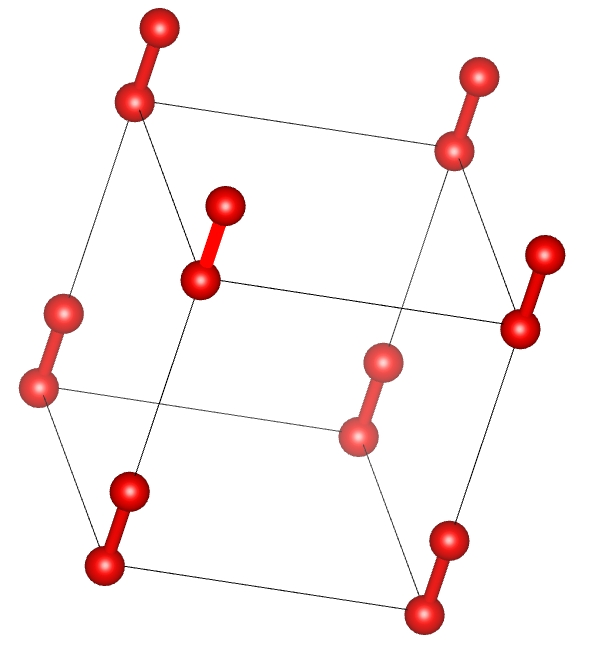
\includegraphics[width=0.5\linewidth]{VASP计算/结构优化/对坐标进行优化/fig/氧气分子.png}
        \caption{氧气分子}
        \label{fig:对坐标进行优化ISIF=2-氧气分子}
    \end{figure}
\end{extend}

\subsection{\code{INCAR}设置}\label{subsec:对坐标进行优化ISIF=2-INCAR设置}

下面是一个简单的\code{INCAR}文件

\begin{lstlisting}[caption=INCAR]
ENCUT  =  600
LWAVE  = .FALSE.
LCHARG = .FALSE.
PREC   = Accurate
NSW    =  300
ISMEAR =  0
SIGMA  =  0.05
IBRION =  2
ISIF   =  2
EDIFFG = -0.01
\end{lstlisting}

\begin{itemize}
    \item \code{ENCUT}:截断能(单位:eV),根据所使用的\code{POTCAR}文件所决定,需要大于所使用\code{POTCAR}当中所有元素\code{ENMAX}的最大值,且通常至少为1.3倍的\code{ENMAX}。在本例中我们设置为600 eV;
    \item \code{LWAVE}和\code{LCHARG}:是否输出\code{WAVECAR}和\code{CHGCAR}文件(分别为波函数和电荷密度)。由于结构优化时通常不关心这些文件,因此设置为\code{.FALSE.}节省硬盘空间;
    \item \code{PREC}:计算精度,在进行结构优化时,为确保结构合理,通常设置为\code{Accurate};
    \item \code{NSW}:离子弛豫的最大步数。如\ref{subsec:为什么要进行结构优化-结构优化原理}中所介绍的那样,结构优化需要进行多步离子弛豫直到收敛。若离子弛豫步数达到\code{NSW}则直接停止(哪怕没有收敛);
    \item \code{ISMEAR}:决定在布里渊区积分时,如何计算分布函数。当设置为0时表示使用Gaussian展宽,其展宽宽度由\code{SIGMA}参数决定(单位:eV);
    \item \code{ISIF}:设置为2表示仅优化原子坐标,不优化晶格;
    \item \code{EDIFFG}:当设置为正值时表示能量收敛标准,当设置为负值时表示原子之间的作用力收敛标准。
\end{itemize}

在本例中,我们设置\code{ISIF=2},这是由于我们所优化的结构为分子体系,并不希望优化外面的晶格参数。除此之外,\code{ISIF}还有其他参数(常见的可能设置为3,在下一节介绍)。同时,通过设置\code{EDIFFG}决定收敛精度,通常设置为\code{-0.01}就已经达到了一般研究所需要的精度,但对于更高精度需求(例如计算声子谱),则可能需要到\code{-1E-3}的精度。

在实际使用时,可以考虑使用VASPKIT,使用\code{vaspkit-101-LR}或者\code{vaspkit-101-SR},其中前者默认设置\code{ISIF=3},而后者设置\code{ISIF=2}

\subsection{其他输入文件}\label{subsec:对坐标进行优化ISIF=2-其他输入文件}

由于计算的是分子体系,不需要考虑周期性,因此在计算时\code{KPOINTS}的设置仅使用Gamma点即可。在生成时可以使用\code{vaspkit-102-2-0}生成Gamma点的\code{KPOINTS}。调用这个命令的同时也会生成默认的\code{POTCAR}文件。

\subsection{计算结果分析}\label{subsec:对坐标进行优化ISIF=2-计算结果分析}

对于结构优化,我们重点关注\code{OSZICAR}和\code{CONTCAR}文件。执行上面的任务,所得到的\code{OSZICAR}文件如下所示(仅供参考):

(为排版方便,对小数点进行了截断处理)

\begin{lstlisting}[caption=OSZICAR,basicstyle=\tiny]
        N       E                     dE             d eps       ncg     rms          rms(c)
DAV:   1     0.281908272337E+02    0.28191E+02   -0.56622E+03   192   0.105E+02
DAV:   2    -0.903395442264E+01   -0.37225E+02   -0.37218E+02   288   0.201E+01
DAV:   3    -0.907739062911E+01   -0.43436E-01   -0.43400E-01   192   0.111E+00
DAV:   4    -0.907742563069E+01   -0.35002E-04   -0.35001E-04   384   0.308E-02
DAV:   5    -0.907742563010E+01    0.58537E-09   -0.20560E-10   192   0.244E-05    0.457E+00
DAV:   6    -0.882350546712E+01    0.25392E+00   -0.36319E-01   288   0.584E-01    0.232E+00
DAV:   7    -0.876665612077E+01    0.56849E-01   -0.21667E-01   288   0.455E-01    0.528E-01
DAV:   8    -0.876722043380E+01   -0.56431E-03   -0.29377E-03   192   0.633E-02    0.946E-02
DAV:   9    -0.876743337124E+01   -0.21294E-03   -0.36429E-04   192   0.156E-02    0.840E-02
DAV:  10    -0.876745195297E+01   -0.18582E-04   -0.10996E-04   384   0.396E-03
    1 F= -.87674520E+01 E0= -.87392430E+01  d E =-.876745E+01
        N       E                     dE             d eps       ncg     rms          rms(c)
DAV:   1    -0.808025287647E+01    0.68718E+00   -0.16093E+02   192   0.127E+01    0.305E+00
DAV:   2    -0.795453762419E+01    0.12572E+00   -0.39880E-01   192   0.592E-01    0.127E+00
DAV:   3    -0.794549043084E+01    0.90472E-02   -0.60348E-02   192   0.231E-01    0.485E-01
DAV:   4    -0.794766566379E+01   -0.21752E-02   -0.75618E-03   288   0.399E-02    0.116E+00
DAV:   5    -0.794386208834E+01    0.38036E-02   -0.20840E-03   192   0.313E-02    0.976E-02
DAV:   6    -0.794680317652E+01   -0.29411E-02   -0.26287E-04   192   0.224E-02    0.617E-02
DAV:   7    -0.794688859816E+01   -0.85422E-04   -0.60875E-05   384   0.439E-03
    2 F= -.79468886E+01 E0= -.79186800E+01  d E =0.820563E+00
        N       E                     dE             d eps       ncg     rms          rms(c)
DAV:   1    -0.889539988611E+01   -0.94860E+00   -0.11596E+02   192   0.109E+01    0.256E+00
DAV:   2    -0.881026749441E+01    0.85132E-01   -0.25112E-01   192   0.539E-01    0.109E+00
DAV:   3    -0.880256066279E+01    0.77068E-02   -0.51306E-02   288   0.214E-01    0.822E-01
DAV:   4    -0.880096355131E+01    0.15971E-02   -0.13725E-02   192   0.253E-02    0.593E-01
DAV:   5    -0.880239330538E+01   -0.14298E-02   -0.25530E-03   192   0.526E-02    0.508E-02
DAV:   6    -0.880262470351E+01   -0.23140E-03   -0.19288E-04   192   0.153E-02    0.654E-02
DAV:   7    -0.880264094151E+01   -0.16238E-04   -0.68975E-05   192   0.261E-03
    3 F= -.88026409E+01 E0= -.87744321E+01  d E =-.351890E-01
        N       E                     dE             d eps       ncg     rms          rms(c)
DAV:   1    -0.880299916057E+01   -0.37446E-03   -0.21780E-02   192   0.152E-01    0.391E-02
DAV:   2    -0.880298590664E+01    0.13254E-04   -0.11371E-04   288   0.121E-02
    4 F= -.88029859E+01 E0= -.87747765E+01  d E =-.355340E-01
        N       E                     dE             d eps       ncg     rms          rms(c)
DAV:   1    -0.880299994411E+01   -0.78354E-06   -0.94840E-04   192   0.314E-02    0.592E-02
DAV:   2    -0.880305353569E+01   -0.53592E-04   -0.50512E-04   192   0.455E-03
    5 F= -.88030535E+01 E0= -.87748689E+01  d E =-.356016E-01    
\end{lstlisting}

其中每一个\code{DAV}开头的行表示\emph{电子步},当电子步达到收敛条件时则会计算\emph{离子步}。在本例中,程序一共计算了5个离子步而达到收敛条件,从而结束计算。

\begin{extend}
    在本例中,我们没有提供电子步的收敛条件。在VASP中,电子步的收敛是由\code{EDIFF}参数决定,默认为\code{1E-4},单位为eV。
\end{extend}

\begin{attention}
    由于\code{NSW}参数,对于一些复杂的或者初始结构不合理的结构,有可能计算离子步达到\code{NSW}所设置的最大值仍未收敛。因此,可以通过查看\code{OUTCAR}文件中是否输出“reached required accuracy - stopping structural energy minimisation”从而确定结构优化是否收敛。

    可以使用\code{grep "reached required" OUTCAR}命令查看。
\end{attention}

结构优化的结果在\code{CONTCAR}文件中,你可以将其复制为\code{POSCAR}进行后续计算,也可以将其导出至如VESTA软件进行可视化分析。本例所计算得到的\code{CONTCAR}如下所示(仅供参考):

\begin{lstlisting}[caption=CONTCAR]
O2                                      
    1.000000000000000     
     5.0000000000000000    0.0000000000000000    0.0000000000000000
     0.0000000000000000    5.0000000000000000    0.0000000000000000
     0.0000000000000000    0.0000000000000000    5.0000000000000000
   O 
     2
Direct
 -0.0000000005038475  0.0000000006063874 -0.0030779335361196
  0.0000000005038475 -0.0000000006063874  0.2445779335361217
 
  0.00000000E+00  0.00000000E+00  0.00000000E+00
  0.00000000E+00  0.00000000E+00  0.00000000E+00
\end{lstlisting}

\begin{extend}
    相较于\code{POSCAR},\code{CONTCAR}多输出了一部分(如上述文件中的最后两行)。它表示每个原子的初始速度,用于计算分子动力学(AIMD)。通常情况下,全部设置为0表示\emph{静力学计算}。
\end{extend}